\section{Supplementary Human Connectome Project Results}
\label{sec:supp_CI_figs}

\begin{table}[htbp]
\hspace*{-0.5cm}
\begin{adjustbox}{center}
\centering
    \begin{tabular}{cm{50mm}m{50mm}m{50mm}}
       \toprule
         Threshold $c$ & \hspace{1.4cm} Sagittal (X = 61) & \ \hspace{1.2cm} Coronal (Y = 75) & \hspace{1.0cm} Axial (Z = 37)\\
        \midrule
        1.0\% BOLD change & 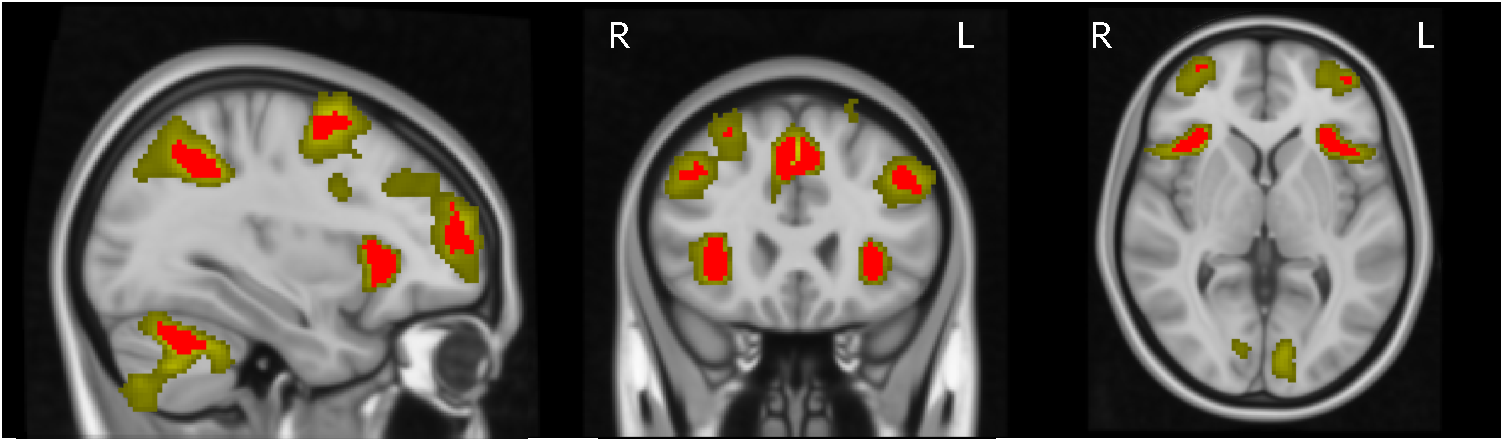
\includegraphics[height=45mm]{CIB_GLM_Fig1_c10.pdf}\\
        1.5\% BOLD change & 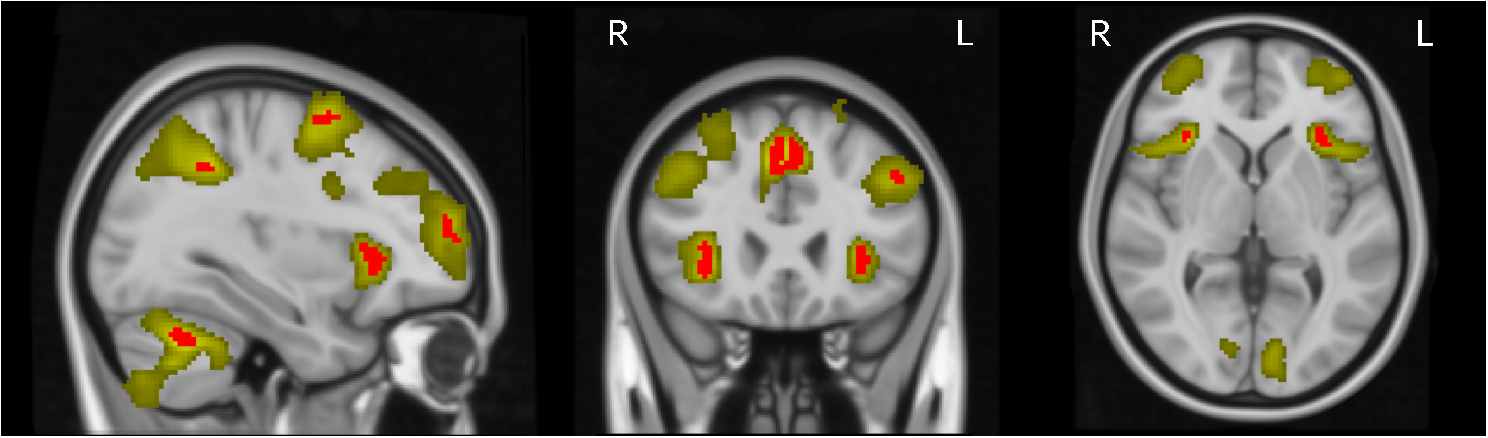
\includegraphics[height=45.5mm]{CIB_GLM_Fig1_c15.pdf}\\
        2.0\% BOLD change & 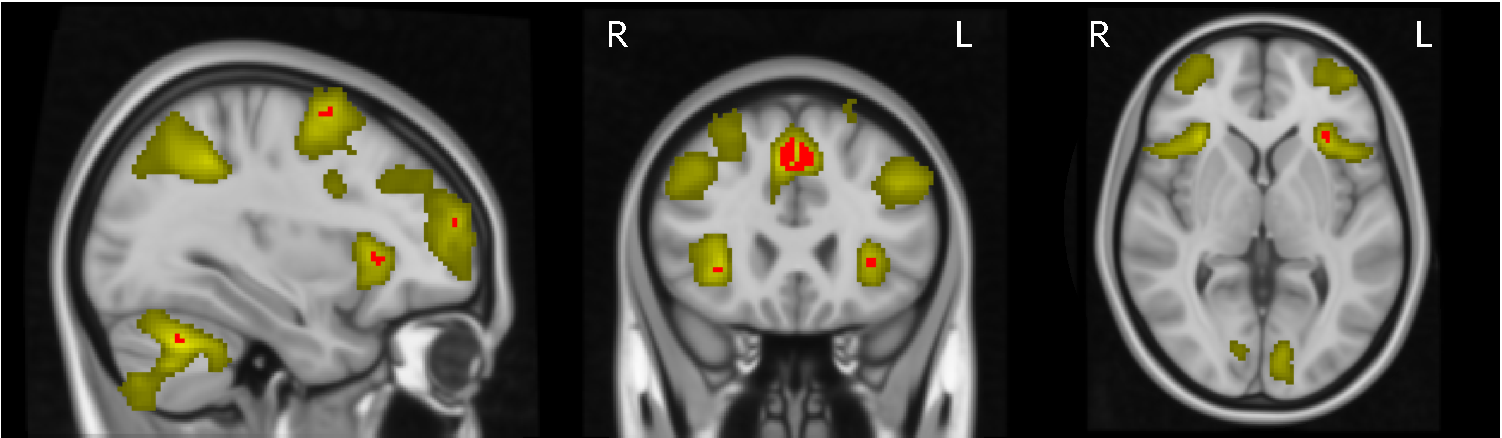
\includegraphics[height=45mm]{CIB_GLM_Fig1_c20.pdf}\\
        \bottomrule
    \end{tabular}
\end{adjustbox}
    \captionof{figure}{Comparing the upper Confidences Sets for the HCP working memory task data (same slice views as Fig. \ref{tbl:HCP_results_one}) with the thresholded $t$-statistic results obtained by applying a traditional group-level one-sample $t$-test, voxelwise $p < 0.05$ FWE correction (green-yellow voxels). While over 25,000 voxels were determined as statistically significant with the standard inference method, less than 5,000 voxels were asserted to have at least a 1.0\% BOLD change by the CSs. In particular, the two statistically significant clusters spanning the left and right side of the frontal lobe contained almost no voxels with a practical effect size of over 1.5\% BOLD change.}
    \label{tbl:Supp_HCP_results_one}
\end{table}

\begin{table}[htbp]
\hspace*{-0.5cm}
\begin{adjustbox}{center}
\centering
    \begin{tabular}{cm{50mm}m{50mm}m{50mm}}
       \toprule
         Threshold $c$ & \hspace{1.4cm} Sagittal (X = 47) & \ \hspace{1.2cm} Coronal (Y = 71) & \hspace{1.0cm} Axial (Z = 60)\\
        \midrule
        1.0\% BOLD change & 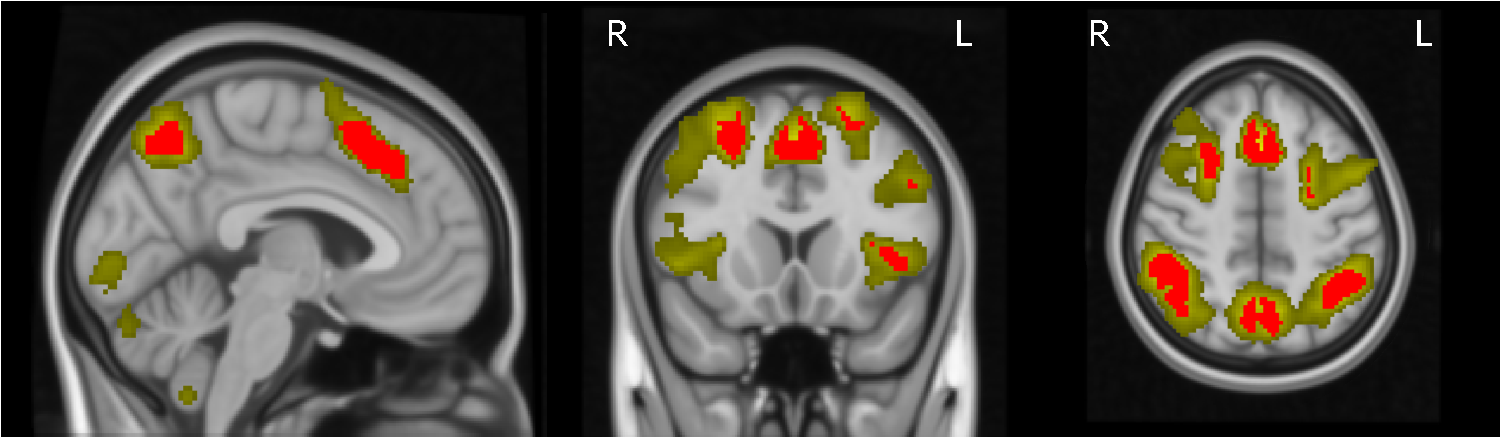
\includegraphics[height=45mm]{CIB_GLM_Fig2_c10.pdf}\\
        1.5\% BOLD change & 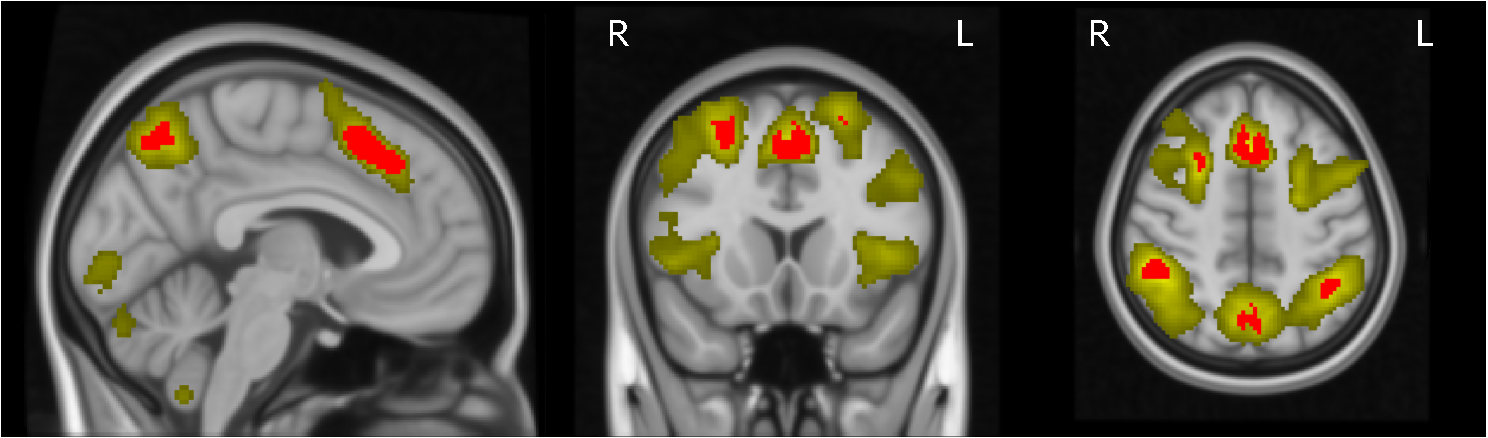
\includegraphics[height=45.5mm]{CIB_GLM_Fig2_c15.pdf}\\
        2.0\% BOLD change & 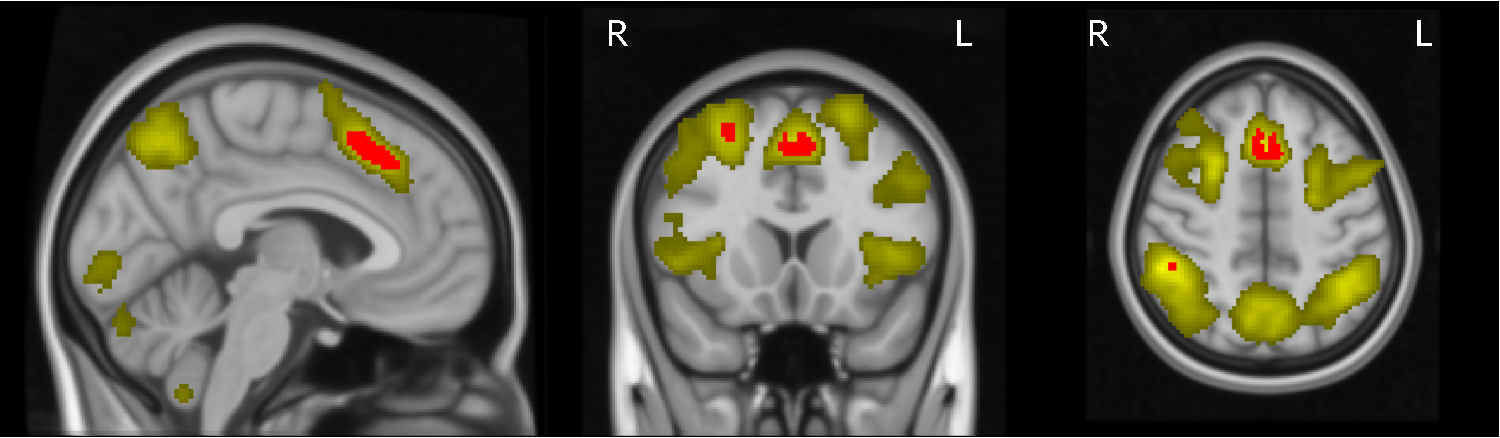
\includegraphics[height=45mm]{CIB_GLM_Fig2_c20.pdf}\\
        \bottomrule
    \end{tabular}
\end{adjustbox}
    \captionof{figure}{Comparing the upper Confidences Sets for the HCP working memory task data (same slice views as Fig. \ref{tbl:HCP_results_two}) with the thresholded $t$-statistic results obtained by applying a traditional group-level one-sample $t$-test, voxelwise $p < 0.05$ FWE correction (green-yellow voxels). While one large statistically significant cluster covers the supramarginal gyrus, angular gyrus and precuneous, the CSs localize the precise areas with practically significant effect sizes within each of these regions.}
    \label{tbl:Supp_HCP_results_two}
\end{table}

\section{Supplementary Tables}
\label{sec:supp_CI_tabs}

\begin{table}[htbp]
\vspace{-5.0em}
\caption{Empirical coverage results for the 2D simulations using nominal (nom.) coverage levels $1-\alpha = 80\%, 90\%$ and $95\%$. Results are shown for applying the Wild $t$-Bootstrap method to the residual field along the estimated boundary $\dAhatc$ (top) and the true boundary $\dAc$ (bottom).}
\centering
\hspace*{-1.5cm}
\begin{tabular}{@{}p{0.14\textwidth}*{4}{L{\dimexpr0.26\textwidth-2\tabcolsep\relax}}@{}}
\toprule
& \multicolumn{2}{c}{\textbf{2D Signal 1. (Ramp)}} &
\multicolumn{2}{c}{\textbf{2D Signal 2. (Circle)}} \\
\cmidrule(r{4pt}){2-3} \cmidrule(l){4-5}
& \textbf{Standard Dev 1.} & \ \textbf{Standard Dev 2.} & \ \ \textbf{Standard Dev 1.} & \ \textbf{Standard Dev 2.}\\
\midrule
$\mathbf{\dAhatc}$  \\[-0.4em]
$80\%$ nom.  \\[-0.4em]
$N = \hphantom{1}60$ & 90.13\% $\pm$ 0.54\% & 87.57\% $\pm$ 0.60\% & 78.13\% $\pm$ 0.75\% & 80.23\% $\pm$ 0.73\% \\[-0.4em]
$\hphantom{N{}={}}120$ & 87.53\% $\pm$ 0.60\% & 88.40\% $\pm$ 0.58\% & 80.53\% $\pm$ 0.72\% & 78.70\% $\pm$ 0.75\% \\[-0.4em]
$\hphantom{N{}={}}240$ & 87.43\% $\pm$ 0.61\% & 87.33\% $\pm$ 0.61\% & 79.73\% $\pm$ 0.73\% & 79.53\% $\pm$ 0.74\% \\[-0.4em]
$\hphantom{N{}={}}480$ & 87.40\% $\pm$ 0.61\% & 85.07\% $\pm$ 0.65\% & 78.50\% $\pm$ 0.75\% & 77.40\% $\pm$ 0.76\%\\
$90\%$ nom.  \\[-0.4em]
$N = \hphantom{1}60$ & 95.53\% $\pm$ 0.38\% & 94.83\% $\pm$ 0.40\% & 88.90\% $\pm$ 0.57\% & 89.90\% $\pm$ 0.55\% \\[-0.4em]
$\hphantom{N{}={}}120$ & 94.07\% $\pm$ 0.43\% & 93.73\% $\pm$ 0.44\% & 90.13\% $\pm$ 0.54\% & 89.40\% $\pm$ 0.56\% \\[-0.4em]
$\hphantom{N{}={}}240$ & 94.23\% $\pm$ 0.43\% & 93.60\% $\pm$ 0.45\% & 89.17\% $\pm$ 0.57\% & 90.17\% $\pm$ 0.54\% \\[-0.4em]
$\hphantom{N{}={}}480$ & 93.50\% $\pm$ 0.45\% & 93.33\% $\pm$ 0.46\% & 89.30\% $\pm$ 0.56\% & 88.40\% $\pm$ 0.58\%\\ 
$95\%$ nom.  \\[-0.4em]
$N = \hphantom{1}60$ & 97.67\% $\pm$ 0.28\% & 97.33\% $\pm$ 0.29\% & 94.10\% $\pm$ 0.43\% & 94.60\% $\pm$ 0.41\% \\[-0.4em]
$\hphantom{N{}={}}120$ & 97.13\% $\pm$ 0.30\% & 96.60\% $\pm$ 0.33\% & 94.40\% $\pm$ 0.42\% & 94.37\% $\pm$ 0.42\% \\[-0.4em]
$\hphantom{N{}={}}240$ & 97.30\% $\pm$ 0.30\% & 97.07\% $\pm$ 0.31\% & 94.43\% $\pm$ 0.42\% & 95.53\% $\pm$ 0.38\% \\[-0.4em]
$\hphantom{N{}={}}480$ & 96.97\% $\pm$ 0.31\% & 97.13\% $\pm$ 0.30\% & 94.80\% $\pm$ 0.41\% & 93.73\% $\pm$ 0.44\%\\
\midrule
$\mathbf{\dAc}$\\[-0.4em]
$80\%$ nom.\\[-0.4em]
$N = \hphantom{1}60$ & 60.27\% $\pm$ 0.89\% & 57.30\% $\pm$ 0.90\% & 78.17\% $\pm$ 0.75\% & 80.23\% $\pm$ 0.73\% \\[-0.4em]
$\hphantom{N{}={}}120$ & 66.03\% $\pm$ 0.86\% & 68.30\% $\pm$ 0.85\% & 80.53\% $\pm$ 0.72\% & 78.67\% $\pm$ 0.75\%\\[-0.4em]
$\hphantom{N{}={}}240$ & 71.10\% $\pm$ 0.83\% & 72.23\% $\pm$ 0.82\% & 79.83\% $\pm$ 0.73\% & 79.57\% $\pm$ 0.74\% \\[-0.4em]
$\hphantom{N{}={}}480$ & 76.27\% $\pm$ 0.78\% & 76.17\% $\pm$ 0.78\% & 78.57\% $\pm$ 0.75\% & 77.40\% $\pm$ 0.76\%\\ 
$90\%$ nom.  \\[-0.4em]
$N = \hphantom{1}60$ & 78.47\% $\pm$ 0.75\% & 76.60\% $\pm$ 0.77\% & 88.97\% $\pm$ 0.57\% & 90.00\% $\pm$ 0.55\% \\[-0.4em]
$\hphantom{N{}={}}120$ & 81.67\% $\pm$ 0.71\% & 83.40\% $\pm$ 0.68\% & 90.20\% $\pm$ 0.54\% & 89.43\% $\pm$ 0.56\% \\[-0.4em]
$\hphantom{N{}={}}240$ & 85.20\% $\pm$ 0.65\% & 85.83\% $\pm$ 0.64\% & 89.17\% $\pm$ 0.57\% & 90.17\% $\pm$ 0.54\% \\[-0.4em]
$\hphantom{N{}={}}480$ & 88.50\% $\pm$ 0.58\% & 87.23\% $\pm$ 0.61\% & 89.27\% $\pm$ 0.57\% & 88.43\% $\pm$ 0.58\%\\ 
$95\%$ nom.  \\[-0.4em]
$N = \hphantom{1}60$ & 88.97\% $\pm$ 0.57\% & 87.27\% $\pm$ 0.61\% & 94.17\% $\pm$ 0.43\% & 94.57\% $\pm$ 0.41\% \\[-0.4em]
$\hphantom{N{}={}}120$ & 89.87\% $\pm$ 0.55\% & 90.67\% $\pm$ 0.53\% & 94.47\% $\pm$ 0.42\% & 94.30\% $\pm$ 0.42\% \\[-0.4em]
$\hphantom{N{}={}}240$ & 92.07\% $\pm$ 0.49\% & 92.47\% $\pm$ 0.48\% & 94.40\% $\pm$ 0.42\% & 95.50\% $\pm$ 0.39\% \\[-0.4em]
$\hphantom{N{}={}}480$ & 94.23\% $\pm$ 0.43\% & 94.10\% $\pm$ 0.43 \% & 94.87\% $\pm$ 0.40\% & 93.73\% $\pm$ 0.44\%\\
\bottomrule
\end{tabular}
\label{tbl:supp_CI_2D_results}
\end{table}

\pagebreak

\begin{table}[htbp]
\vspace{-5.0em}
\caption{Empirical coverage results for the 3D simulations using nominal (nom.) coverage levels $1-\alpha = 80\%, 90\%$ and $95\%$. Results are shown for applying the Wild $t$-Bootstrap method to the residual field along the estimated boundary $\dAhatc$ (top) and the true boundary $\dAc$ (bottom).}
\centering
\hspace*{-1.5cm}
\begin{tabular}{@{}p{0.14\textwidth}*{4}{L{\dimexpr0.26\textwidth-2\tabcolsep\relax}}@{}}
\toprule
& \multicolumn{2}{c}{\textbf{3D Signal 1. (Small Sphere)}} &
\multicolumn{2}{c}{\textbf{3D Signal 2. (Large Sphere)}} \\
\cmidrule(r{4pt}){2-3} \cmidrule(l){4-5}
& \textbf{Standard Dev 1.} & \ \textbf{Standard Dev 2.} & \ \ \textbf{Standard Dev 1.} & \ \textbf{Standard Dev 2.}\\
\midrule
$\mathbf{\dAhatc}$  \\[-0.4em]
$80\%$ nom.  \\[-0.4em]
$N = \hphantom{1}60$ & 83.40\% $\pm$ 0.68\% & 83.77\% $\pm$ 0.67\% & 85.10\% $\pm$ 0.65\% & 85.73\% $\pm$ 0.64\% \\[-0.4em]
$\hphantom{N{}={}}120$ & 83.67\% $\pm$ 0.67\% & 84.03\% $\pm$ 0.67\% & 85.87\% $\pm$ 0.64\% & 85.23\% $\pm$ 0.65\% \\[-0.4em]
$\hphantom{N{}={}}240$ & 84.03\% $\pm$ 0.67\% & 83.77\% $\pm$ 0.67\% & 85.23\% $\pm$ 0.65\% & 85.40\% $\pm$ 0.64\% \\[-0.4em]
$\hphantom{N{}={}}480$ & 85.03\% $\pm$ 0.65\% & 82.20\% $\pm$ 0.70\% & 87.67\% $\pm$ 0.60\% & 85.30\% $\pm$ 0.65\%\\
$90\%$ nom.  \\[-0.4em]
$N = \hphantom{1}60$ & 92.30\% $\pm$ 0.49\% & 92.87\% $\pm$ 0.47\% & 92.40\% $\pm$ 0.48\% & 93.47\% $\pm$ 0.45\% \\[-0.4em]
$\hphantom{N{}={}}120$ & 92.07\% $\pm$ 0.49\% & 91.27\% $\pm$ 0.52\% & 93.00\% $\pm$ 0.47\% & 93.50\% $\pm$ 0.45\% \\[-0.4em]
$\hphantom{N{}={}}240$ & 92.33\% $\pm$ 0.49\% & 92.87\% $\pm$ 0.47\% & 93.30\% $\pm$ 0.46\% & 92.90\% $\pm$ 0.47\% \\[-0.4em]
$\hphantom{N{}={}}480$ & 93.03\% $\pm$ 0.46\% & 91.53\% $\pm$ 0.51\% & 93.50\% $\pm$ 0.45\% & 93.47\% $\pm$ 0.45\%\\ 
$95\%$ nom.  \\[-0.4em]
$N = \hphantom{1}60$ & 96.87\% $\pm$ 0.32\% & 96.83\% $\pm$ 0.32\% & 96.40\% $\pm$ 0.34\% & 96.70\% $\pm$ 0.33\% \\[-0.4em]
$\hphantom{N{}={}}120$ & 96.07\% $\pm$ 0.35\% & 95.60\% $\pm$ 0.37\% & 96.97\% $\pm$ 0.31\% & 97.10\% $\pm$ 0.31\% \\[-0.4em]
$\hphantom{N{}={}}240$ & 96.20\% $\pm$ 0.35\% & 96.83\% $\pm$ 0.32\% & 96.23\% $\pm$ 0.35\% & 96.90\% $\pm$ 0.32\% \\[-0.4em]
$\hphantom{N{}={}}480$ & 96.30\% $\pm$ 0.34\% & 96.13\% $\pm$ 0.35\% & 96.83\% $\pm$ 0.32\% & 93.80\% $\pm$ 0.44\%\\
\midrule
$\mathbf{\dAc}$\\[-0.4em]
$80\%$ nom.\\[-0.4em]
$N = \hphantom{1}60$ & 83.60\% $\pm$ 0.68\% & 83.90\% $\pm$ 0.67\% & 85.20\% $\pm$ 0.65\% & 85.80\% $\pm$ 0.64\% \\[-0.4em]
$\hphantom{N{}={}}120$ & 83.80\% $\pm$ 0.67\% & 83.93\% $\pm$ 0.67\% & 85.90\% $\pm$ 0.64\% & 85.23\% $\pm$ 0.65\%\\[-0.4em]
$\hphantom{N{}={}}240$ & 84.03\% $\pm$ 0.67\% & 83.90\% $\pm$ 0.67\% & 85.27\% $\pm$ 0.65\% & 85.40\% $\pm$ 0.64\% \\[-0.4em]
$\hphantom{N{}={}}480$ & 85.03\% $\pm$ 0.65\% & 82.27\% $\pm$ 0.70\% & 87.73\% $\pm$ 0.60\% & 85.37\% $\pm$ 0.65\%\\ 
$90\%$ nom.  \\[-0.4em]
$N = \hphantom{1}60$ & 92.43\% $\pm$ 0.48\% & 92.90\% $\pm$ 0.47\% & 92.37\% $\pm$ 0.48\% & 93.40\% $\pm$ 0.45\% \\[-0.4em]
$\hphantom{N{}={}}120$ & 91.97\% $\pm$ 0.50\% & 91.43\% $\pm$ 0.51\% & 92.97\% $\pm$ 0.47\% & 93.60\% $\pm$ 0.45\% \\[-0.4em]
$\hphantom{N{}={}}240$ & 92.37\% $\pm$ 0.48\% & 92.90\% $\pm$ 0.47\% & 93.33\% $\pm$ 0.46\% & 92.90\% $\pm$ 0.47\% \\[-0.4em]
$\hphantom{N{}={}}480$ & 93.03\% $\pm$ 0.46\% & 91.40\% $\pm$ 0.51\% & 93.57\% $\pm$ 0.45\% & 93.47\% $\pm$ 045\%\\ 
$95\%$ nom.  \\[-0.4em]
$N = \hphantom{1}60$ & 96.87\% $\pm$ 0.32\% & 96.93\% $\pm$ 0.31\% & 96.37\% $\pm$ 0.34\% & 96.70\% $\pm$ 0.33\% \\[-0.4em]
$\hphantom{N{}={}}120$ & 96.07\% $\pm$ 0.35\% & 95.53\% $\pm$ 0.38\% & 96.97\% $\pm$ 0.31\% & 97.13\% $\pm$ 0.30\% \\[-0.4em]
$\hphantom{N{}={}}240$ & 96.17\% $\pm$ 0.35\% & 96.93\% $\pm$ 0.31\% & 96.23\% $\pm$ 0.35\% & 96.80\% $\pm$ 0.32\% \\[-0.4em]
$\hphantom{N{}={}}480$ & 96.33\% $\pm$ 0.34\% & 96.13\% $\pm$ 0.35\% & 96.77\% $\pm$ 0.32\% & 96.80\% $\pm$ 0.32\% \\
\bottomrule
\end{tabular}
\label{tbl:supp_CI_3D_results}
\end{table}

\begin{table}[htbp]
\vspace{-5.0em}
\caption*{\textbf{Table 2. (continued)}}
\centering
\hspace*{-1.5cm}
\begin{tabular}{@{}p{0.14\textwidth}*{4}{L{\dimexpr0.26\textwidth-2\tabcolsep\relax}}@{}}
\toprule
& \multicolumn{2}{c}{\textbf{3D Signal 3. (Multiple Spheres)}} &
\multicolumn{2}{c}{\textbf{3D Signal 4. (UK Biobank)}} \\
\cmidrule(r{4pt}){2-3} \cmidrule(l){4-5}
& \textbf{Standard Dev 1.} & \ \textbf{Standard Dev 2.} & \textbf{UK Biobank SD} \\
\midrule
$\mathbf{\dAhatc}$  \\[-0.4em]
$80\%$ nom.  \\[-0.4em]
$N = \hphantom{1}60$ & 89.47\% $\pm$ 0.56\% & 89.20\% $\pm$ 0.57\% & 89.17\% $\pm$ 0.57\% &  \\[-0.4em]
$\hphantom{N{}={}}120$ & 87.60\% $\pm$ 0.60\% & 88.17\% $\pm$ 0.59\% & 87.17\% $\pm$ 0.61\% & \\[-0.4em]
$\hphantom{N{}={}}240$ & 86.17\% $\pm$ 0.63\% & 86.33\% $\pm$ 0.63\% & 86.27\% $\pm$ 0.63\% & \\[-0.4em]
$\hphantom{N{}={}}480$ & 86.13\% $\pm$ 0.63\% & 86.10\% $\pm$ 0.63\% & 87.67\% $\pm$ 0.60\%\\ 
$90\%$ nom.  \\[-0.4em]
$N = \hphantom{1}60$ & 95.20\% $\pm$ 0.39\% & 94.87\% $\pm$ 0.40\% & 95.23\% $\pm$ 0.39\% & \\[-0.4em]
$\hphantom{N{}={}}120$ & 94.53\% $\pm$ 0.42\% & 93.97\% $\pm$ 0.43\% & 94.63\% $\pm$ 0.41\% & \\[-0.4em]
$\hphantom{N{}={}}240$ & 93.67\% $\pm$ 0.44\% & 93.17\% $\pm$ 0.46\% & 93.73\% $\pm$ 0.44\% & \\[-0.4em]
$\hphantom{N{}={}}480$ & 93.97\% $\pm$ 0.43\% & 93.87\% $\pm$ 0.44\% & 93.50\% $\pm$ 0.45\%\\ 
$95\%$ nom.  \\[-0.4em]
$N = \hphantom{1}60$ & 97.93\% $\pm$ 0.26\% & 97.73\% $\pm$ 0.27\% & 97.37\% $\pm$ 0.29\% & \\[-0.4em]
$\hphantom{N{}={}}120$ & 97.37\% $\pm$ 0.29\% & 97.47\% $\pm$ 0.29\% & 97.73\% $\pm$ 0.27\% & \\[-0.4em]
$\hphantom{N{}={}}240$ & 97.23\% $\pm$ 0.30\% & 96.50\% $\pm$ 0.34\% & 96.93\% $\pm$ 0.31\% & \\[-0.4em]
$\hphantom{N{}={}}480$ & 97.23\% $\pm$ 0.30\% & 97.63\% $\pm$ 0.28\% & 96.83\% $\pm$ 0.32\%\\
\midrule
$\mathbf{\dAc}$\\[-0.4em]
$80\%$ nom.\\[-0.4em]
$N = \hphantom{1}60$ & 84.30\% $\pm$ 0.66\% & 85.33\% $\pm$ 0.65\% & 83.30\% $\pm$ 0.68\% & \\[-0.4em]
$\hphantom{N{}={}}120$ & 84.93\% $\pm$ 0.65\% & 86.20\% $\pm$ 0.63\% & 85.13\% $\pm$ 0.65\% & \\[-0.4em]
$\hphantom{N{}={}}240$ & 85.73\% $\pm$ 0.64\% & 85.60\% $\pm$ 0.64\% & 84.97\% $\pm$ 0.65\% & \\[-0.4em]
$\hphantom{N{}={}}480$ & 86.03\% $\pm$ 0.63\% & 85.97\% $\pm$ 0.63\% & 87.73\% $\pm$ 0.60\%\\ 
$90\%$ nom.  \\[-0.4em]
$N = \hphantom{1}60$ & 92.93\% $\pm$ 0.47\% & 92.20\% $\pm$ 0.49\% & 92.77\% $\pm$ 0.47\% & \\[-0.4em]
$\hphantom{N{}={}}120$ & 93.20\% $\pm$ 0.46\% & 93.27\% $\pm$ 0.46\% & 93.50\% $\pm$ 0.45\% & \\[-0.4em]
$\hphantom{N{}={}}240$ & 93.37\% $\pm$ 0.45\% & 93.07\% $\pm$ 0.46\% & 92.67\% $\pm$ 0.48\% & \\[-0.4em]
$\hphantom{N{}={}}480$ & 93.97\% $\pm$ 0.43\% & 93.80\% $\pm$ 0.44\% & 93.57\% $\pm$ 0.45\%\\ 
$95\%$ nom.  \\[-0.4em]
$N = \hphantom{1}60$ & 96.80\% $\pm$ 0.32\% & 96.50\% $\pm$ 0.34\% & 96.70\% $\pm$ 0.33\% & \\[-0.4em]
$\hphantom{N{}={}}120$ & 96.90\% $\pm$ 0.32\% & 96.83\% $\pm$ 0.32\% & 97.07\% $\pm$ 0.31\% & \\[-0.4em]
$\hphantom{N{}={}}240$ & 97.20\% $\pm$ 0.30\% & 96.30\% $\pm$ 0.34\% & 96.40\% $\pm$ 0.34\% & \\[-0.4em]
$\hphantom{N{}={}}480$ & 97.27\% $\pm$ 0.30\% & 97.63\% $\pm$ 0.28\% & 96.77\% $\pm$ 0.32\%\\
\bottomrule
\end{tabular}
\end{table}